%
%\usepackage{tabularx} % extra features for tabular environment
%\usepackage{amsmath}  % improve math presentation
%\usepackage{graphicx} % takes care of graphic including machinery
%\usepackage[margin=1in,letterpaper]{geometry} % decreases margins
%\usepackage[utf8]{inputenc}
%%\usepackage{cite} % takes care of citations
%\usepackage[USenglish]{babel}
%\usepackage[utf8]{inputenc}
%
%\usepackage[backend=biber]{biblatex}
%\usepackage{csquotes}

%
%
%
%\usepackage[final]{hyperref} % adds hyper links inside the generated pdf file
%\hypersetup{
%	colorlinks=true,       % false: boxed links; true: colored links
%	linkcolor=blue,        % color of internal links
%	citecolor=blue,        % color of links to bibliography
%	filecolor=magenta,     % color of file links
%	urlcolor=blue         
%}
%

%++++++++++++++++++++++++++++++++++++++++


%\begin{document}

\title{Git Assignment - CS 6000}
\author{L. Babyak}
\date{September 15, 2020}
\maketitle

\section{Section 1}

My name is Lori Babyak.  I am a first year Computer Science PhD student at the University of Colorado, Colorado Springs. I hold a Bachelor's Degree in Computer Science from UT Austin and a Master's degree, also in Computer Science, from Texas State University. My goals for this course - CS 6000 Computer Science Research Methods- are to learn to research, read, and eventually produce research papers on subjects of interest in Computer Science. Additionally, I am looking forward to getting to know other students in the class and work collaboratively towards goals. Something personal about myself is that I have three grown children, two of whom live in the Denver area. Also, I took an extended vacation with a couple of friends in August. We visited Colorado Springs, Wyoming and South Dakota. In South Dakota, we visited Mt. Rushmore, the Crazy Horse Sculpture, and Custer State Park - where we saw free-roaming bison in their natural environment. I am happy and excited to be part of the UCCS community, and my hope is to make significant contributions to the field.

\begin{figure} [h!]
    \centering
    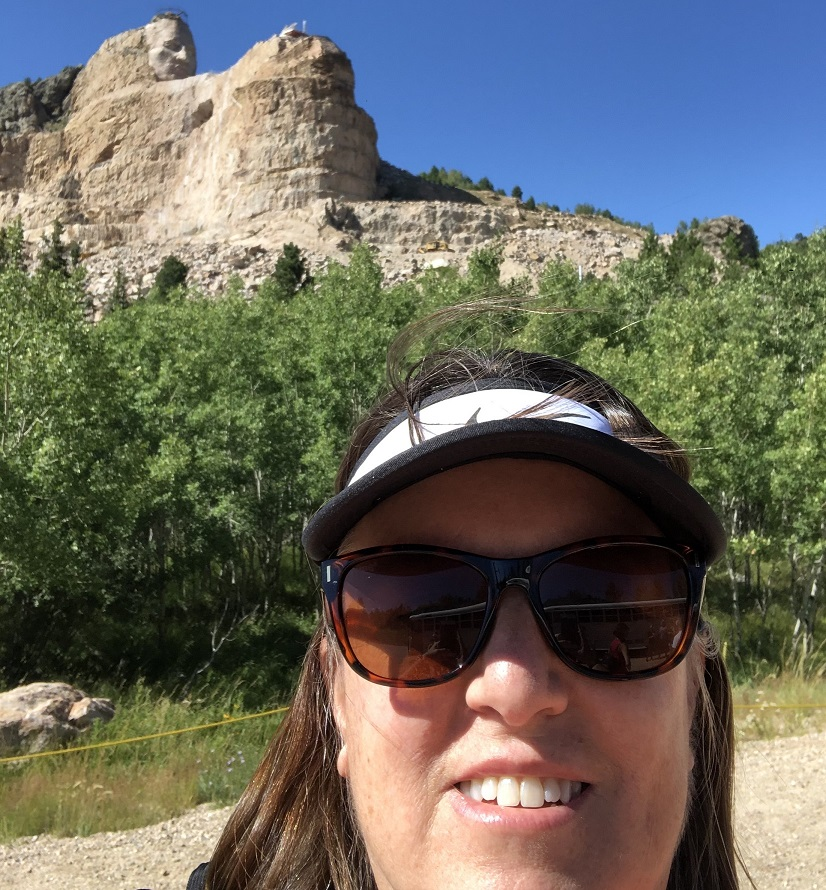
\includegraphics[width=.4\textwidth]{LoriSDSmall.JPG} 
    \caption{A photo of Lori Babyak in front of Crazy Horse sculpture, outside Custer, SD, August 2020}
\end{figure}


\textbf{Question  to Lori Babyak from Constance Hendrix}:  I traveled to Wyoming and South Dakota in July.  Did you have the chance to see Devils Tower?
\textbf{Answer to Question from Constance Hendrix}: We drove through Wyoming and stopped in Torrington.  We only had a couple of days in SD, so we visited Mt. Rushmore, the Crazy Horse Sculpture and Custer State Park.  I don't think we saw Devil's Tower. There's so much to see there!

\textbf{Question from Jackie}
Hi Lori, thanks for sharing. I went to those places twice. The first time was in 2013, and the second time was in 2018. To be honest, I did not see much progress on the Crazy Horse. My questions would be: since you are in Colorado Springs, are you going to snow ski? If you already did, how much you enjoy the mountain views at the top? the cog train is a fun ride, too. 

